\section{Multimedia Representation and Perception}




\begin{questionbox}{Domanda 1}
Explain the \textbf{Contrast Sensitivity Function} (\textbf{CSF}): what it is, in which units \textbf{spatial frequency} is measured, where it peaks, and the direct implication for \textbf{quantization} in compression.
\end{questionbox}


The \textbf{Contrast Sensitivity Function} describes how sensitive the human visual system is to luminance contrast as \textbf{spatial frequency} changes. \textbf{spatial frequency} is measured in cycles per degree of visual angle.

Sensitivity is high at intermediate frequencies and lower at very low and very high frequencies. The usual qualitative curve is band-pass: the eye is less sensitive to very fine high-frequency texture and to very slow luminance variations.

For compression, this justifies frequency-dependent \textbf{quantization}: coefficients corresponding to less visible spatial frequencies can be quantized more coarsely, while visually important frequencies should receive smaller \textbf{quantization} steps.



\begin{questionbox}{Domanda 2}
Compare \textbf{cones} and \textbf{rods} (number, function, lighting conditions) and explain why the RGB-to-Y conversion weights the green component the most.
\end{questionbox}


\textbf{rods} are very sensitive to light intensity and dominate vision in low-light conditions, but they do not provide color perception. \textbf{cones} work in brighter conditions and provide color perception. The three cone classes are sensitive mainly to short, medium and long wavelengths.

The luminance component is a weighted sum of RGB, for example in BT.601:


$$
Y \approx 0.299R + 0.587G + 0.114B
$$


Green receives the largest weight because the human visual system is most sensitive to luminance variations in the green/yellow part of the spectrum. Therefore, preserving green contributes more to perceived brightness detail than preserving blue with the same weight.



\begin{questionbox}{Domanda 3}
Explain the J:a:b \textbf{\textbf{chroma} subsampling} notation. Compute the data-reduction factor of 4:2:0 vs full RGB and justify why it is perceptually acceptable.
\end{questionbox}


The notation $J:a:b$ describes how many \textbf{chroma} samples are kept relative to $J$ \textbf{luma} samples across two image rows. $J$ is the horizontal \textbf{luma} reference, $a$ is the number of \textbf{chroma} samples in the first row, and $b$ is the number of \textbf{chroma} samples in the second row.

For 4:2:0, \textbf{luma} $Y$ is kept at full resolution, while $Cb$ and $Cr$ are sampled at half horizontal and half vertical resolution. Over a $2\times 2$ block:

\begin{itemize}
  \item full RGB \textbf{HAS} $4\times3=12$ component samples;
  \item YCbCr 4:2:0 \textbf{HAS} $4Y+1Cb+1Cr=6$ component samples.
\end{itemize}

So, with the same \textbf{bit depth}, 4:2:0 uses about half the component samples of full RGB. This is perceptually acceptable because the eye is much more sensitive to luminance detail than to chrominance detail.



\begin{questionbox}{Domanda 4}
Draw the Basic Tools for Compression scheme (Transform -> Prediction -> \textbf{quantization} -> \textbf{entropy} Coding) and indicate which stage is the only \textbf{lossy} one and why.
\end{questionbox}


A generic compression chain combines decorrelation, approximation and \textbf{lossless} coding:

\begin{figure}[H]
\centering
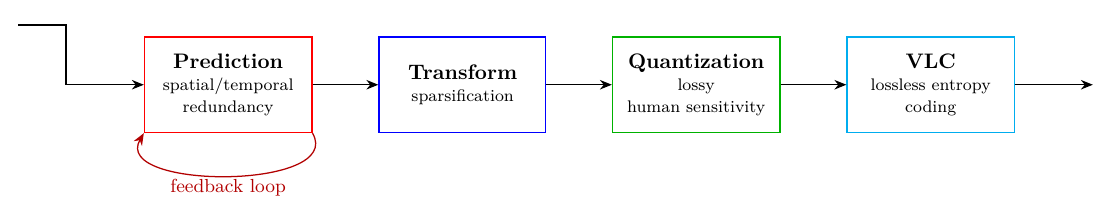
\includegraphics[width=0.75\textwidth]{images/Pasted_image_20260624205627.png}
\caption{Pasted image 20260624205627}
\end{figure}\begin{tcolorbox}[colback=white, colframe=gray!50, height=4.5cm, sharp corners]
\end{tcolorbox}

Prediction and transform reduce redundancy or concentrate energy. \textbf{entropy} coding is \textbf{lossless}: it only assigns shorter codes to more probable symbols.

\textbf{quantization} is the only \textbf{lossy} step because many input values are mapped to the same reconstruction value. This reduces \textbf{rate}, but the original value cannot be recovered exactly.

---


